% Copyright (c) 2014,2016 Casper Ti. Vector
% Public domain.

\chapter{文獻探討}
%\pkuthssffaq % 中文测试文字。
	\section{比特幣(Bitcoin)}
	比特幣(Bitcoin,BTC)是一個點對點式的點子現金系統,集成了非對稱式金鑰密碼學(Asymmetric Key Cryptography)\parencite{AsymmetricKeyCryptography}、簽章密碼學(Signature cryptography)、零知識證明密碼學(Zero Knowledge Proof Cryptography)\parencite{Zero-KnowledgeProofsofIdentity}、哈希函數密碼學(Hash function cryptography)、共式算法(Consensus)諸多技術建構了一個分散式的不需要靠中心化機構加以維護的交易帳本(區塊鏈)。在接下來的章節中將逐一進行詳盡的說明每個技術在各個環節中所扮演的角色。

	\section{比特幣地址}

		\subsection{比特幣地址生成相關函數}
		在點對點的現金系統中,首先必須先生成一個地址,在比特幣的協議中有著既定的程序生成地址。運用到的技術包括亂數產生器、secp256k1\parencite{johnson2001elliptic}、SHA-256(哈希函數)\parencite{DBLP:conf/fse/KhovratovichRS12}、RIPEMD-160(哈希函數)\parencite{DBLP:conf/isw/MendelPRR06}、Base58\parencite{base58}。接下來回詳細說明每一個函數的運做過程以及意義,最後說明比特幣交易地址生成的每一個步驟。
		\subsubsection{亂數產生器(Random number generator)}
		亂數在密碼學中是個相當重要的一環,在比特幣系統中更是重要,畢竟生成的亂數會變成比特幣的私鑰,私鑰是簽署資產轉移的唯一方式,在比特幣地址中的亂數產生器會產出一個256bit長度的亂數,也就是私鑰,256bit的長度可以表現的組態空間為$2^{256}$,換算成十進位表示為$1.1579209x10^{77}$,要在這組態空間中亂數產生同樣的一把私鑰是一件困難的事,但也有國際的實驗室也有團隊正在努力的窮舉比特幣$2^{256}$的組態空間。

		如何建構一個亂數,在過往的亂數產生器往往會加入時間作為參數,但對於一個攻擊者而言,只需要去猜測在這段時間內所有的可能性即可猜出亂數。而亂數在密碼學中通常會是一個把私鑰的構建,在https協議中,服務器端與客戶端,建立一個加密連線的過程中也需要一個亂數去建立一個高安全性的加密通道,在SSH協議中也採用了亂數。
	
		在過去的歷史事件中,發現Android手機版以及平板版的亂數產生器的存在著不隨機,於2013年8月比特幣開發者Mike Hearn提及“All private keys generated on Android phones/tablets are weak and some signatures have been observed to have colliding R values” \parencite{SomeSecureRandomThoughts},Bitcoin.org也發布了警告\parencite{AndroidSecurityVulnerability}簡要說明該事件的原因,以及表明影響到的Bitcoin Wallet 客戶端有Bitcoin Wallet、BitcoinSpinner、Mycelium Bitcoin Wallet、blockchain.info。這樣的錯誤源於Android本身支持的亂數產生器並不隨機,隨後Android解釋了亂數的問題並加以修正。在這Android手機亂數不夠亂的事件中,有自願者自發性地公佈自己的損失狀態,總金額為55.82152538個比特幣\parencite{Badsignaturesleading},但因為比特幣屬於被動的性質,無人主動回報既不會加入統計中,所以總損失應該會超過55.82152538個比特幣。

		\subsubsection{secp256k1}
		\subsubsection{SHA-256}
		\subsubsection{RIPEMD-160}
		\subsubsection{Base58}

	\subsection{比特幣地址生成過程}
		\subsubsection{生成私鑰}
		\subsubsection{生成公鑰}
		\subsubsection{生成公鑰SHA-256}
		\subsubsection{生成公鑰SHA-256的RIPEMD-160}
		\subsubsection{對公鑰SHA-256的RIPEMD-160再做兩次SHA-256前32bit的值作為校驗碼}
		\subsubsection{取得版本號}
		\subsubsection{版本號、公鑰SHA-256的RIPEMD-160和校驗碼合併}
		\subsubsection{合併的結果以Base58編碼}

	\subsection{多重簽名(Multi-Signature)}
		\subsubsection{多重簽名地址}
		\subsubsection{Green Address}

	\section{區塊鏈(Blockchain)}
	%區塊頭所有的結構
		\subsection{Block Header}
			\subsubsection{}

	%區塊內容 交易手續費攻擊
		\subsection{Block Data}

	\section{工作量證明(Proof of Work)}
	\section{點對點網路(Peer to peer network)}

	去中心化的密碼貨幣系統帶給社會帶給傳統的中心化的金融體系以及政府帶來了很重大的衝擊,中本聰建構了一個不需要中央銀行發行貨幣的貨幣系統,在比特幣的貨幣發行上全靠區塊鏈既定的算法。除了貨幣發行,也將交易紀錄的帳本已明文的方式儲存在去中心化的區塊鏈中,以比特幣為例,現今的完整的比特幣區塊鏈帳本已經高達180GB,這樣保存完整交易資料的計算機稱之為全節點,在比特幣去中心化的網路中,如圖\ref{bitcoinfullnode}所示,截至2018年1月25比特幣網路中全節點數量為10552個\parencite{bitcoinfullnode},全節點的數量決定了比特幣帳本的可靠度,倘若有著更多的全結點,會使得比特幣網路堅不可摧,更難去修改歷史發生過的交易數據。

	\begin{figure}
		\centering
		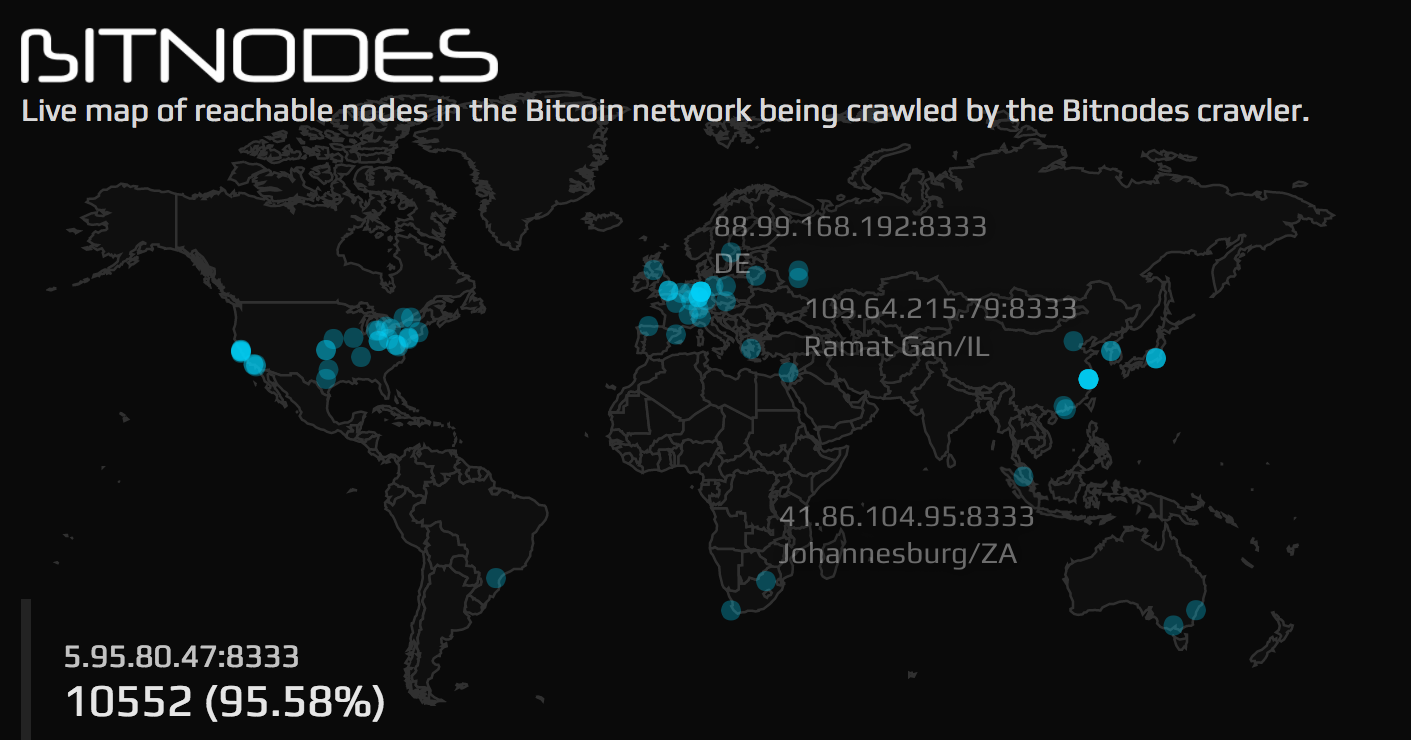
\includegraphics[width = .9\textwidth]{bitcoinfullnode.png}
		\caption{Bitcoin Full Node\parencite{bitcoinfullnode}}\label{bitcoinfullnode}
	\end{figure}

	\section{山寨幣(Altcoin)簡介}

		\subsection{萊特幣(Litecoin)}

		\subsection{狗幣(Dogecoin)}

		\subsection{域名幣(Namecoin)}

		\subsection{以太坊(Etherum)}

% vim:ts=4:sw=4
